%
% Complete documentation on the extended LaTeX markup used for Insight
% documentation is available in ``Documenting Insight'', which is part
% of the standard documentation for Insight.  It may be found online
% at:
%
%     http://www.itk.org/

\documentclass{InsightArticle}

\usepackage[dvips]{graphicx}
\usepackage{float}
\usepackage{filecontents}

\begin{filecontents}{shortbib.bib}
@ARTICLE{reconstruction,
    AUTHOR={M. Kazhdan and M. Bolitho and H. Hoppe},
    TITLE={Poisson Surface Reconstruction},
    JOURNAL={Eurographics Symposium on Geometry Processing},
    YEAR={2006},
}
\end{filecontents}

\usepackage{subfigure}

%%%%%%%%%%%%%%%%%%%%%%%%%%%%%%%%%%%%%%%%%%%%%%%%%%%%%%%%%%%%%%%%%%
%
%  hyperref should be the last package to be loaded.
%
%%%%%%%%%%%%%%%%%%%%%%%%%%%%%%%%%%%%%%%%%%%%%%%%%%%%%%%%%%%%%%%%%%
\usepackage[dvips,
bookmarks,
bookmarksopen,
backref,
colorlinks,linkcolor={blue},citecolor={blue},urlcolor={blue},
]{hyperref}


\title{Poisson Surface Reconstruction for VTK}

% 
% NOTE: This is the last number of the "handle" URL that 
% The Insight Journal assigns to your paper as part of the
% submission process. Please replace the number "1338" with
% the actual handle number that you get assigned.
%
\newcommand{\IJhandlerIDnumber}{3149}

% Increment the release number whenever significant changes are made.
% The author and/or editor can define 'significant' however they like.
\release{0.00}

% At minimum, give your name and an email address.  You can include a
% snail-mail address if you like.

\author{David Doria \and Arnaud Gelas}
\authoraddress{Rensselaer Polytechnic Institute, Troy NY \and Harvard Medical School, Boston MA}

\begin{document}

%
% Add hyperlink to the web location and license of the paper.
% The argument of this command is the handler identifier given
% by the Insight Journal to this paper.
% 
\IJhandlefooter{\IJhandlerIDnumber}


\ifpdf
\else
   %
   % Commands for including Graphics when using latex
   % 
   \DeclareGraphicsExtensions{.eps,.jpg,.gif,.tiff,.bmp,.png}
   \DeclareGraphicsRule{.jpg}{eps}{.jpg.bb}{`convert #1 eps:-}
   \DeclareGraphicsRule{.gif}{eps}{.gif.bb}{`convert #1 eps:-}
   \DeclareGraphicsRule{.tiff}{eps}{.tiff.bb}{`convert #1 eps:-}
   \DeclareGraphicsRule{.bmp}{eps}{.bmp.bb}{`convert #1 eps:-}
   \DeclareGraphicsRule{.png}{eps}{.png.bb}{`convert #1 eps:-}
\fi


\maketitle


\ifhtml
\chapter*{Front Matter\label{front}}
\fi


% The abstract should be a paragraph or two long, and describe the
% scope of the document.
\begin{abstract}
\noindent
This document presents an implementation of the Poission surface reconstruction algorithm in the VTK framework. (This code was adapted directly from the original implementation by Misha Kazhdan \cite{reconstruction}, with permission). We present a class, $vtkPoissonReconstruction$, which produces a surface from an oriented point set. A Paraview plugin interface is provided to allow extremely easy experimentation with the new functionality. We propose these classes as an addition to the Visualization Toolkit.

\end{abstract}

\IJhandlenote{\IJhandlerIDnumber}

\tableofcontents

\section{Introduction}
There are several data acquisition methods which produce 3D points as output. Examples include Light Detection and Ranging (LiDAR) scanners, Structure From Motion (SFM) algorithms, and Multi View Stereo (MVS) algorithms. It is often producing a mesh from these points if often of interest. This paper presents a simple algorithm for producing a surface from a set of 3D points which have an associated normal vector. This method was originally published in \cite{reconstruction}, we have simply implemented it in the VTK framework.

\section{vtkPoissonReconstruction}

\subsection{Options}
\subsubsection{Depth}
This integer controls the reconstruction depth; the maximum depth of the tree that will be used for surface reconstruction. Running at depth $d$ corresponds to solving on a voxel grid whose resolution is no larger than $2^d \times 2^d \times 2^d$. Note that since the reconstructor adapts the octree to the sampling density, the specified reconstruction depth is only an upper bound. The default value for this parameter is 8.

This value can be set using:
\begin{verbatim}
reconstructionFilter->SetDepth(10);
\end{verbatim}

\subsubsection{Scale}
This floating point value specifies the ratio between the diameter of the cube used for reconstruction and the diameter of the samples' bounding cube.
The default value is 1.25.

This value can be set using:
\begin{verbatim}
reconstructionFilter->SetScale(1.1); 
\end{verbatim}

\subsubsection{SolverDivide}
Solver subdivision depth; This integer argument specifies the depth at which a block Gauss-Seidel solver is used to solve the Laplacian equation. Using this parameter helps reduce the memory overhead at the cost of a small increase in reconstruction time. (In practice, we have found that for reconstructions of depth 9 or higher a subdivide depth of 7 or 8 can greatly reduce the memory usage.) The default value is 8.

This value can be set using:
\begin{verbatim}
reconstructionFilter->SetSolverDivide(7); 
\end{verbatim}

\subsubsection{IsoDivide}
Iso-surface extraction subdivision depth; This integer argument specifies the depth at which a block iso-surface extractor should be used to extract the iso-surface. Using this parameter helps reduce the memory overhead at the cost of a small increase in extraction time. (In practice, we have found that for reconstructions of depth 9 or higher a subdivide depth of 7 or 8 can greatly reduce the memory usage.) The default value is 8.

This value can be set using:
\begin{verbatim}
reconstructionFilter->SetIsoDivide(9); 
\end{verbatim}

\subsubsection{SamplesPerNode}
Minimum number of samples; This floating point value specifies the minimum number of sample points that should fall within an octree node as the octree construction is adapted to sampling density. For noise-free samples, small values in the range [1.0 - 5.0] can be used. For more noisy samples, larger values in the range [15.0 - 20.0] may be needed to provide a smoother, noise-reduced, reconstruction. The default value is 1.0.

This value can be set using:
\begin{verbatim}
reconstructionFilter->SetSamplesPerNode(1.0); 
\end{verbatim}

\subsubsection{Confidence}
Enabling tells the reconstructor to use the size of the normals as confidence information. When the flag is not enabled, all normals are normalized to have unit-length prior to reconstruction.

This value can be set using:
\begin{verbatim}
reconstructionFilter->SetConfidence(0); 
\end{verbatim}

\subsubsection{Verbose}
Enabling this flag provides a more verbose description of the running times and memory usages of individual components of the surface reconstructor.

This value can be set using:
\begin{verbatim}
reconstructionFilter->SetVerbose(0);
\end{verbatim}


%%%%%%%%%%%%%%%%%%%%%%%%%%%%%%%%%%
\subsection{Demonstration}
To demonstrate Poisson surface reconstruction, we use an oriented point cloud of a horse. This data set is shown in Figure \ref{fig:HorsePoints}. In Figure \ref{fig:HorseSurface}, we show the reconstructed surface.

\begin{figure}[H]
\centering
\subfigure[Horse oriented point set]{
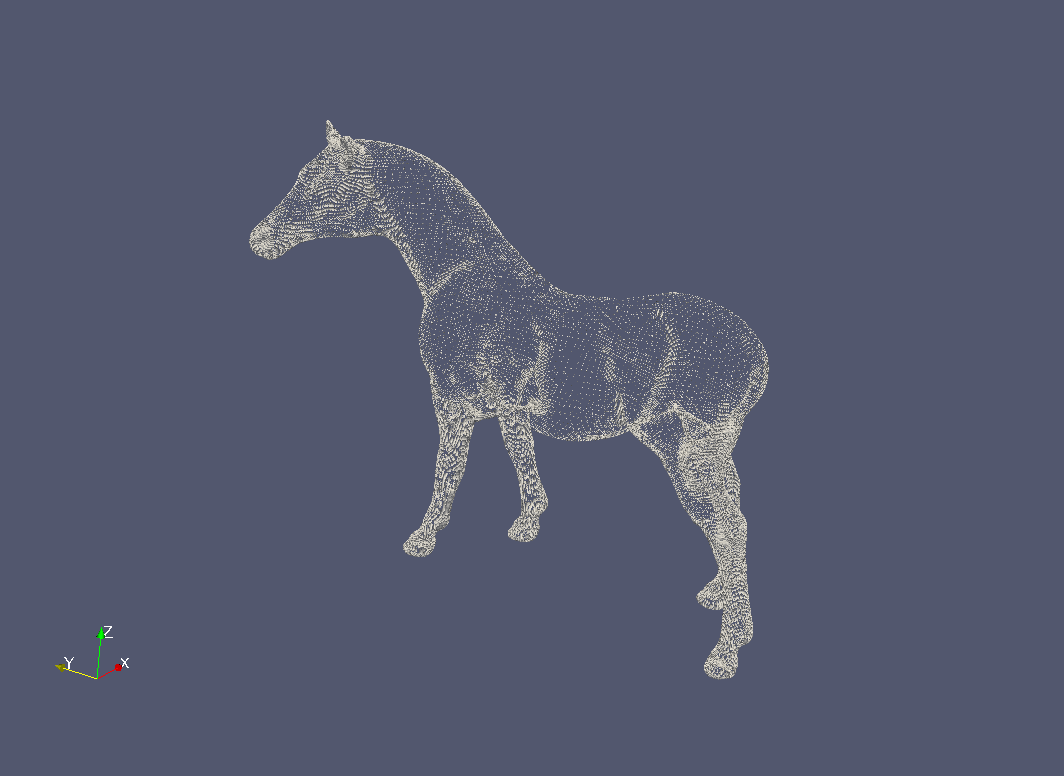
\includegraphics[width=0.3\linewidth]{Images/HorsePoints}
\label{fig:HorsePoints}
}
\subfigure[Horse surface]{
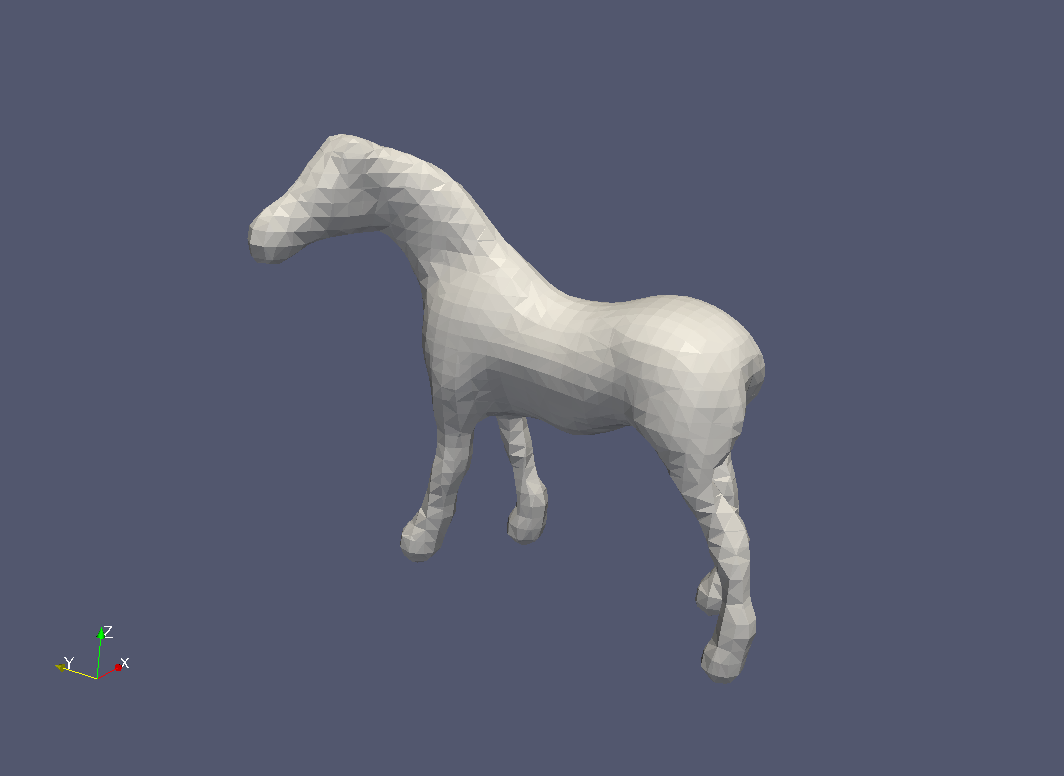
\includegraphics[width=0.3\linewidth]{Images/HorseSurface}
\label{fig:HorseSurface}
}
\caption{Poisson surface reconstruction demonstration.}
\label{fig:SurfaceReconstruction}
\end{figure}

\subsection{Code Snippet}
\begin{verbatim}
vtkSmartPointer<vtkXMLPolyDataReader> reader =
	vtkSmartPointer<vtkXMLPolyDataReader>::New();
reader->SetFileName(inputFileName.c_str());
reader->Update();

vtkSmartPointer<vtkPoissonReconstruction> poissonFilter = 
	vtkSmartPointer<vtkPoissonReconstruction>::New();
poissonFilter->SetDepth( depth );
poissonFilter->SetInputConnection(reader->GetOutputPort());
poissonFilter->Update();
\end{verbatim}

%%%%%%%%%%%%%%%%%%%%%
\pagebreak
\section{Paraview Plugin}
For convenience, this code is shipped with a Paraview filter plugin. The plugin provides an easy way to set the parameters as well as integrate the new code into your workflow. A screenshot of the plugin interface is shown in Figure \ref{fig:Plugin}.

\begin{figure}[H]
\centering
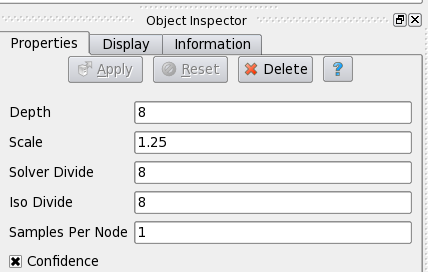
\includegraphics[width=0.3\linewidth]{Images/Plugin}
\label{fig:Plugin}
\caption{Paraview plugin screenshot}
\end{figure}

\bibliographystyle{plain}
\bibliography{shortbib}


\end{document}
